\section{Trabalhos Relacionados}
\label{section:trabalhos_relacionados}

\citeauthoronline{silvio_taynan:2017} (\citeyear{silvio_taynan:2017}) cita 
em seu estudo que a prova de redação do ENEM é avaliada considerando uma matriz 
de referência do \citeauthor{edital_enem:2016} (\citeyear{edital_enem:2016}), 
desenvolvida com a colaboração de especialistas, com o objetivo de 
operacionalizar o exame. A matriz apresenta cinco competências, para cada 
competência expressa para redação existem níveis de conhecimento associados de 
0 a 5. Conforme \citeauthoronline{braga:2015} (\citeyear{braga:2015}) cita na
sua pesquisa, num texto de redação, o candidato defenderá uma opinião a 
respeito do tema proposto, de forma coerente e coesa, apoiado em argumentos 
consistentes. O texto será redigido a respeitar a escrita formal da Língua 
Portuguesa. Ao fim, o candidato elabora uma proposta de intervenção social para 
o problema apresentado no desenvolvimento do texto, respeitando os direitos 
humanos.

Em sua pesquisa \citeauthoronline{monard_baranauskas:2003} 
(\citeyear{monard_baranauskas:2003}) cita: ``A indução é a forma de 
inferência lógica que permite obter conclusões genéricas sobre um conjunto 
particular de exemplos'', ou seja, na indução, um conceito é aprendido 
efetuando-se inferência indutiva sobre as amostras apresentadas. O aprendizado 
indutivo pode ser dividido em supervisionado e não supervisionado como 
ilustrada a Figura \ref{figure:aprendizado_indutivo}. No aprendizado não 
supervisionado, o algoritmo analisa os exemplos fornecidos e tenta determinar 
se alguns deles podem ser agrupados de alguma maneira, formando 
\textit{clusters} ou agrupamentos. Já no aprendizado supervisionado é fornecido 
ao algoritmo de um conjunto de exemplos de treinamento para os quais o rótulo 
da classe associada é conhecido.

\begin{figure}[H]
\begin{center}
    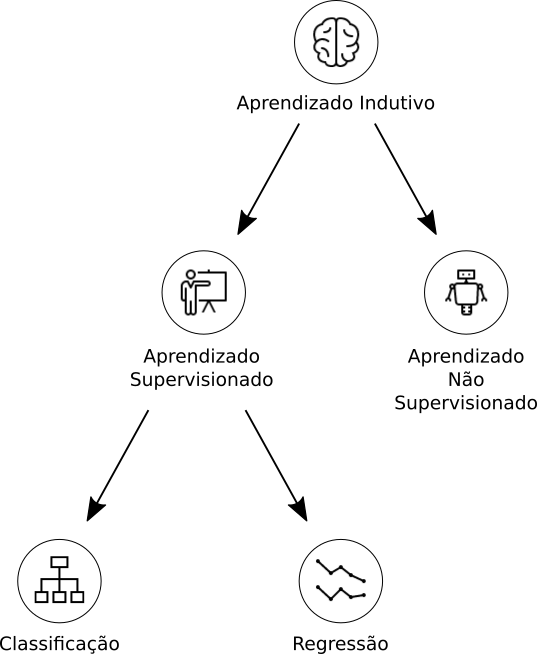
\includegraphics[scale=0.40]{images/aprendizado_indutivo.png}
\end{center}
\caption{Árvore hierárquica do aprendizado indutivo, a qual é dividida em 
algoritmos supervisionado e não-supervisionado.}
\label{figure:aprendizado_indutivo}
\end{figure}

Classificadores são utilizados para a predição de classes de objetos e pode ser 
dito como o processo de generalização dos dados a partir de diferentes 
instâncias. Existe uma tendência de se referir a problemas com respostas 
quantitativas como ``problemas de regressão'' e aqueles com uma saída 
qualitativa como ``problemas de classificação''. Dado um conjunto de exemplos 
como ilustrado na Figura \ref{figure:processo_classificacao}, os 
classificadores devem encontrar uma função geral capaz de prever adequadamente 
as saídas para novas amostras. Após o treinamento, o classificador é avaliado e 
se necessário o processo de classificação pode ser ajustado usando o 
conhecimento sobre o domínio do problema, conforme 
\citeauthoronline{porthos_motta:2016} (\citeyear{porthos_motta:2016}) explica 
na sua pesquisa.

\begin{figure}[H]
\begin{center}
    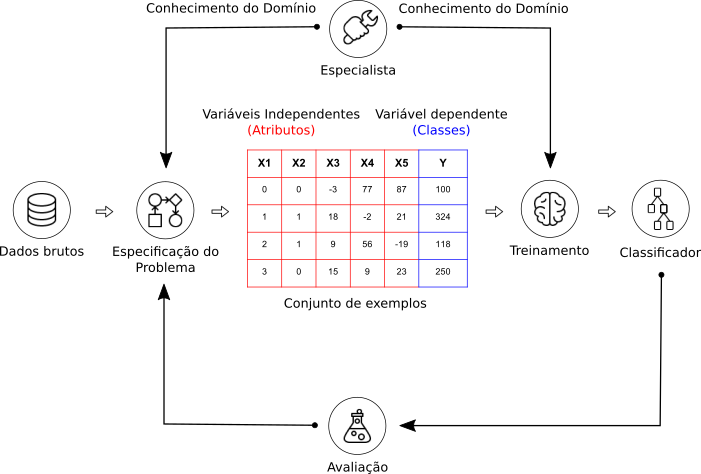
\includegraphics[scale=0.60]{images/processo_classificacao.png}
\end{center}
\caption{Fluxo do processo de classificação, o modelo encontra uma função geral 
capaz de prever as saídas, a especificação do problema pode ser reajustada com 
o conhecimento do domínio para obter um melhor resultado.}
\label{figure:processo_classificacao}
\end{figure}

No processo de mineração de dados, \citeauthoronline{matsubara2003pretext} 
(\citeyear{matsubara2003pretext}), descrevem que na etapa de pré-processamento 
de textos, um dos métodos geralmente adotado é a representação usando a 
abordagem ``bag-of-words'', uma das representações estruturadas mais simples. 
Utiliza técnicas de redução do termo ao seu radical e remoção de termos 
irrelevantes. Cada documento é representado como um vetor de palavras que 
ocorrem no texto, especificamente uma tabela atributo-valor. 

O algoritmo Naive Bayes destaca-se entre os classificadores devido ao seu 
comportamento simplista, traz bons resultados em muitos casos. 
\citeauthoronline{de2017mineraccao} (\citeyear{de2017mineraccao}), cita na sua 
pesquisa o classificador Naive Bayes como um progenitor probabilístico. Baseado 
no Teorema de Bayes, criado por Thomas Bayes no século XVIII, este 
classificador é eleito o mais eficiente na precisão e rotulagem de novas 
amostras, conforme o estudo de \citeauthoronline{chakrabarti2002mining} 
(\citeyear{chakrabarti2002mining}). Naive Bayes desconsidera a correlação entre 
as variáveis (``features''), ou seja, se determinada fruta é considerada uma 
``Maçã'' se ela for ``Vermelha'', ``Redonda'' e possui ``aproximadamente 10 cm 
de diâmetro'', o algoritmo não vai levar em consideração a correlação entre 
esses fatores, tratando cada um de forma independente.

\textit{AdaBoost} ou \textit{Adaptive Boosting}, derivado do \textit{Boosting} 
é um dos algoritmos mais populares no Aprendizado de Máquina. Utiliza uma 
técnica que usa diversos classificadores fracos com a finalidade de aumentar a 
acurácia geral. Segundo \citeauthoronline{dos2015detecccao} 
(\citeyear{dos2015detecccao}), o seu sucesso deve-se ao mérito de conseguir 
adaptar-se aos classificadores de base. Neste algoritmo, os classificadores são 
gerados de forma a ajudar os exemplos incorretamente classificados pelos 
classificadores antecedentes, ele aumenta os pesos dos exemplos em que os 
classificadores anteriores cometeram erros para indicar importância do 
exemplo no conjunto.

\citeauthoronline{junior2017proposta} (\citeyear{junior2017proposta}) propõem 
no seu estudo o desenvolvimento de um sistema para avaliação automática de 
redações, utilizando processamento de linguagem natural, extração de 
características e classificação. O objetivo do sistema é  apresentar uma 
estratégia para redução do esforço no processo de correção e avaliação das 
redações, para isso, no processamento do texto foi eliminado o conjunto de 
termos que eventualmente não trazia significado ao texto, na séquência é 
atribuido marcas (``tags'') morfológicas e de inflexão para cada token do 
texto. Cada redação e representada por um vetor com as seguintes 
características: quantidades de parágrafos, frases, palavras, caracteres, erros 
ortográficos, e erros gramaticais identificados. A partir deste vertor de 
características e realizada a inferência indutiva do classificador SVM 
``Support Vector Machine''. O resultado apresentado é uma acurácia de 0,52 
sobre a classificação da competência I (um) da matriz de referência do 
\citeauthor{edital_enem:2016}.